\documentclass[twoside]{book}

% Packages required by doxygen
\usepackage{calc}
\usepackage{doxygen}
\usepackage{graphicx}
\usepackage[utf8]{inputenc}
\usepackage{makeidx}
\usepackage{multicol}
\usepackage{multirow}
\usepackage{textcomp}
\usepackage[table]{xcolor}

% Font selection
\usepackage[T1]{fontenc}
\usepackage{mathptmx}
\usepackage[scaled=.90]{helvet}
\usepackage{courier}
\usepackage{amssymb}
\usepackage{sectsty}
\renewcommand{\familydefault}{\sfdefault}
\allsectionsfont{%
  \fontseries{bc}\selectfont%
  \color{darkgray}%
}
\renewcommand{\DoxyLabelFont}{%
  \fontseries{bc}\selectfont%
  \color{darkgray}%
}

% Page & text layout
\usepackage{geometry}
\geometry{%
  a4paper,%
  top=2.5cm,%
  bottom=2.5cm,%
  left=2.5cm,%
  right=2.5cm%
}
\tolerance=750
\hfuzz=15pt
\hbadness=750
\setlength{\emergencystretch}{15pt}
\setlength{\parindent}{0cm}
\setlength{\parskip}{0.2cm}
\makeatletter
\renewcommand{\paragraph}{%
  \@startsection{paragraph}{4}{0ex}{-1.0ex}{1.0ex}{%
    \normalfont\normalsize\bfseries\SS@parafont%
  }%
}
\renewcommand{\subparagraph}{%
  \@startsection{subparagraph}{5}{0ex}{-1.0ex}{1.0ex}{%
    \normalfont\normalsize\bfseries\SS@subparafont%
  }%
}
\makeatother

% Headers & footers
\usepackage{fancyhdr}
\pagestyle{fancyplain}
\fancyhead[LE]{\fancyplain{}{\bfseries\thepage}}
\fancyhead[CE]{\fancyplain{}{}}
\fancyhead[RE]{\fancyplain{}{\bfseries\leftmark}}
\fancyhead[LO]{\fancyplain{}{\bfseries\rightmark}}
\fancyhead[CO]{\fancyplain{}{}}
\fancyhead[RO]{\fancyplain{}{\bfseries\thepage}}
\fancyfoot[LE]{\fancyplain{}{}}
\fancyfoot[CE]{\fancyplain{}{}}
\fancyfoot[RE]{\fancyplain{}{\bfseries\scriptsize Generated on Fri Apr 11 2014 20:04:31 for My Project by Doxygen }}
\fancyfoot[LO]{\fancyplain{}{\bfseries\scriptsize Generated on Fri Apr 11 2014 20:04:31 for My Project by Doxygen }}
\fancyfoot[CO]{\fancyplain{}{}}
\fancyfoot[RO]{\fancyplain{}{}}
\renewcommand{\footrulewidth}{0.4pt}
\renewcommand{\chaptermark}[1]{%
  \markboth{#1}{}%
}
\renewcommand{\sectionmark}[1]{%
  \markright{\thesection\ #1}%
}

% Indices & bibliography
\usepackage{natbib}
\usepackage[titles]{tocloft}
\setcounter{tocdepth}{3}
\setcounter{secnumdepth}{5}
\makeindex

% Hyperlinks (required, but should be loaded last)
\usepackage{ifpdf}
\ifpdf
  \usepackage[pdftex,pagebackref=true]{hyperref}
\else
  \usepackage[ps2pdf,pagebackref=true]{hyperref}
\fi
\hypersetup{%
  colorlinks=true,%
  linkcolor=blue,%
  citecolor=blue,%
  unicode%
}

% Custom commands
\newcommand{\clearemptydoublepage}{%
  \newpage{\pagestyle{empty}\cleardoublepage}%
}


%===== C O N T E N T S =====

\begin{document}

% Titlepage & ToC
\hypersetup{pageanchor=false}
\pagenumbering{roman}
\begin{titlepage}
\vspace*{7cm}
\begin{center}%
{\Large My Project }\\
\vspace*{1cm}
{\large Generated by Doxygen 1.8.4}\\
\vspace*{0.5cm}
{\small Fri Apr 11 2014 20:04:31}\\
\end{center}
\end{titlepage}
\clearemptydoublepage
\tableofcontents
\clearemptydoublepage
\pagenumbering{arabic}
\hypersetup{pageanchor=true}

%--- Begin generated contents ---
\chapter{Hierarchical Index}
\section{Class Hierarchy}
This inheritance list is sorted roughly, but not completely, alphabetically\-:\begin{DoxyCompactList}
\item \contentsline{section}{Magic\-Square\-Set}{\pageref{classMagicSquareSet}}{}
\item \contentsline{section}{Square}{\pageref{classSquare}}{}
\begin{DoxyCompactList}
\item \contentsline{section}{Magic\-Square}{\pageref{classMagicSquare}}{}
\end{DoxyCompactList}
\end{DoxyCompactList}

\chapter{Class Index}
\section{Class List}
Here are the classes, structs, unions and interfaces with brief descriptions\-:\begin{DoxyCompactList}
\item\contentsline{section}{\hyperlink{classCoinSlot}{Coin\-Slot} }{\pageref{classCoinSlot}}{}
\item\contentsline{section}{\hyperlink{structDestination}{Destination} }{\pageref{structDestination}}{}
\item\contentsline{section}{\hyperlink{classDestinationCollection}{Destination\-Collection} }{\pageref{classDestinationCollection}}{}
\item\contentsline{section}{\hyperlink{classPriceComputer}{Price\-Computer} }{\pageref{classPriceComputer}}{}
\item\contentsline{section}{\hyperlink{classRefoundComputer}{Refound\-Computer} }{\pageref{classRefoundComputer}}{}
\item\contentsline{section}{\hyperlink{classTicketMachine}{Ticket\-Machine} }{\pageref{classTicketMachine}}{}
\end{DoxyCompactList}

\chapter{Class Documentation}
\hypertarget{classBuch}{\section{Buch Class Reference}
\label{classBuch}\index{Buch@{Buch}}
}
Inheritance diagram for Buch\-:\begin{figure}[H]
\begin{center}
\leavevmode
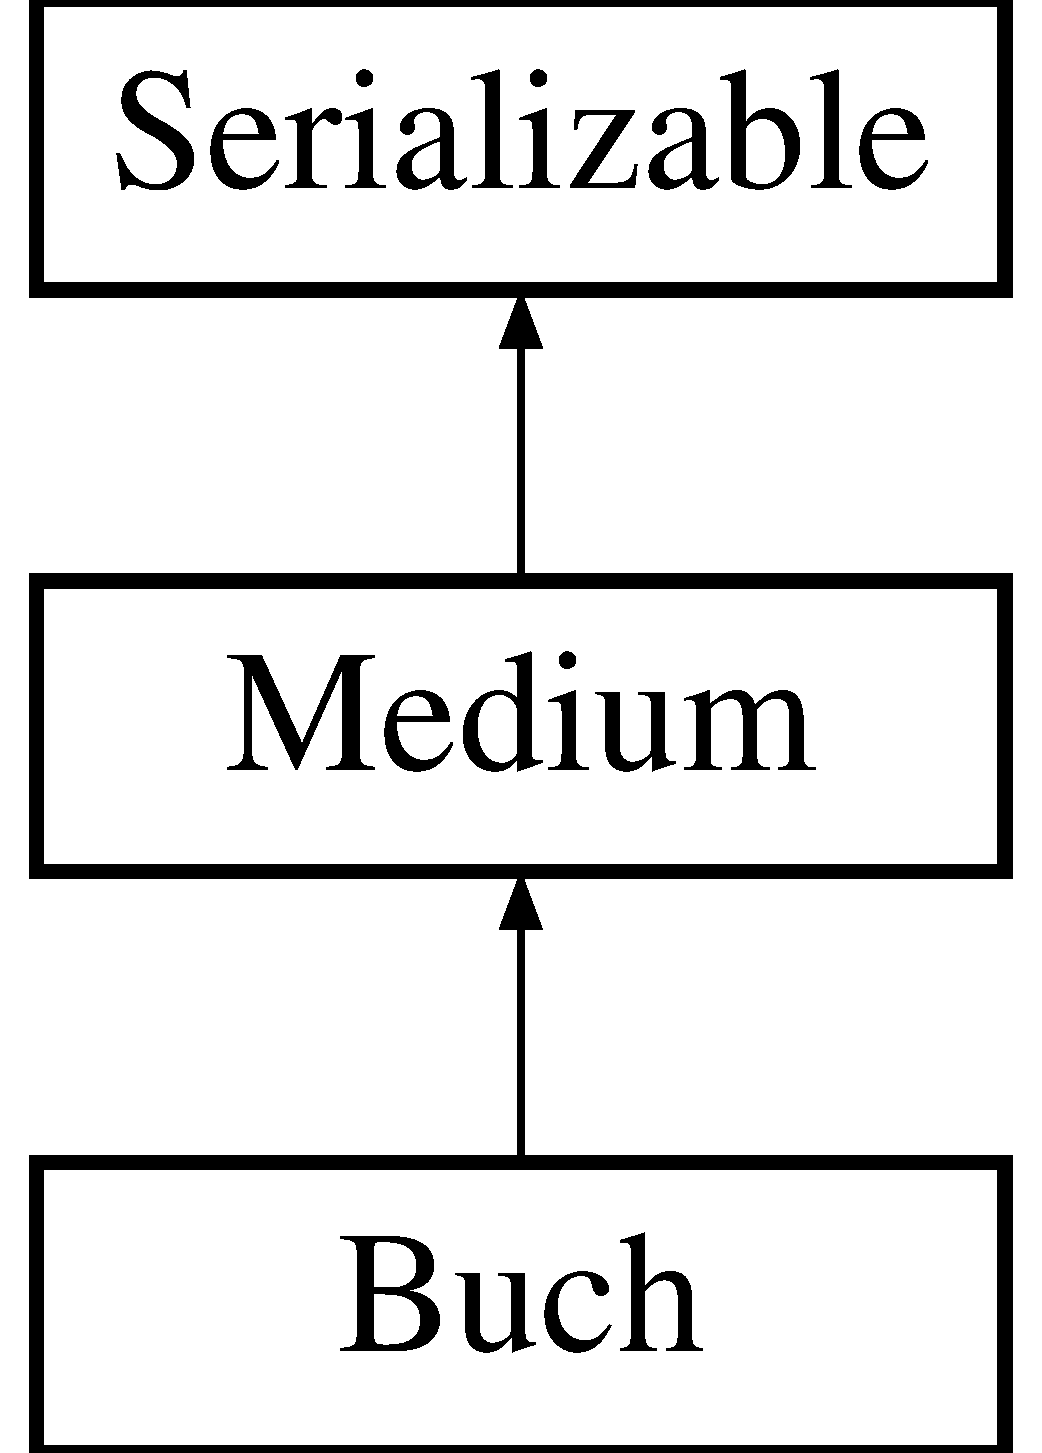
\includegraphics[height=3.000000cm]{classBuch}
\end{center}
\end{figure}
\subsection*{Public Member Functions}
\begin{DoxyCompactItemize}
\item 
\hyperlink{classBuch_ad7e7857afc44de2527a626f700d9ec48}{Buch} (String titel, float preis, String author, boolean hardcover)
\item 
\hyperlink{classBuch_ad45d958a80f07ea2cb5cb564b5fd2254}{Buch} (Random random)
\item 
\hypertarget{classBuch_a4c8bf45949dcf36734951c7aeee4868b}{String {\bfseries gib\-Author} ()}\label{classBuch_a4c8bf45949dcf36734951c7aeee4868b}

\item 
void \hyperlink{classBuch_a92311208a213dfb8b8feea909269ee98}{setze\-Author} (String author)
\item 
boolean \hyperlink{classBuch_a8707574befbe4b23f44ee1ca52b90d59}{gib\-Hardcover} ()
\item 
void \hyperlink{classBuch_a364e47149d84b52313f6222de0d1eb1e}{setze\-Hardcover} (boolean hardcover)
\item 
String \hyperlink{classBuch_ac0d79c56b86295a71110e0437d4d0bfc}{to\-String} ()
\end{DoxyCompactItemize}


\subsection{Detailed Description}
\hyperlink{classBuch}{Buch} ist eine Unterklasse von \hyperlink{classMedium}{Medium}. Es ergänzt \hyperlink{classMedium}{Medium} mit den für ein \hyperlink{classBuch}{Buch} benötigten Felder und Eigenschaften.

\begin{DoxyAuthor}{Author}
Lukas Hodel 
\end{DoxyAuthor}


\subsection{Constructor \& Destructor Documentation}
\hypertarget{classBuch_ad7e7857afc44de2527a626f700d9ec48}{\index{Buch@{Buch}!Buch@{Buch}}
\index{Buch@{Buch}!Buch@{Buch}}
\subsubsection[{Buch}]{\setlength{\rightskip}{0pt plus 5cm}Buch.\-Buch (
\begin{DoxyParamCaption}
\item[{String}]{titel, }
\item[{float}]{preis, }
\item[{String}]{author, }
\item[{boolean}]{hardcover}
\end{DoxyParamCaption}
)\hspace{0.3cm}{\ttfamily [inline]}}}\label{classBuch_ad7e7857afc44de2527a626f700d9ec48}
Der Konstruktor benoetigt alle Felder des Buches als Parameter


\begin{DoxyParams}{Parameters}
{\em titel} & String Titel des Buches. \\
\hline
{\em preis} & Float Preis des Buches. \\
\hline
{\em author} & String Author des Buches. \\
\hline
{\em hardcover} & boolean ob hardcover oder nicht. \\
\hline
\end{DoxyParams}
\hypertarget{classBuch_ad45d958a80f07ea2cb5cb564b5fd2254}{\index{Buch@{Buch}!Buch@{Buch}}
\index{Buch@{Buch}!Buch@{Buch}}
\subsubsection[{Buch}]{\setlength{\rightskip}{0pt plus 5cm}Buch.\-Buch (
\begin{DoxyParamCaption}
\item[{Random}]{random}
\end{DoxyParamCaption}
)\hspace{0.3cm}{\ttfamily [inline]}}}\label{classBuch_ad45d958a80f07ea2cb5cb564b5fd2254}
Der Konstruktor benoetigt ein Random Objekt, dann werden die Felder automatisch gefüllt.


\begin{DoxyParams}{Parameters}
{\em random} & Objekt zur zufaelligen Wertegerierung. \\
\hline
\end{DoxyParams}


\subsection{Member Function Documentation}
\hypertarget{classBuch_a8707574befbe4b23f44ee1ca52b90d59}{\index{Buch@{Buch}!gib\-Hardcover@{gib\-Hardcover}}
\index{gib\-Hardcover@{gib\-Hardcover}!Buch@{Buch}}
\subsubsection[{gib\-Hardcover}]{\setlength{\rightskip}{0pt plus 5cm}boolean Buch.\-gib\-Hardcover (
\begin{DoxyParamCaption}
{}
\end{DoxyParamCaption}
)\hspace{0.3cm}{\ttfamily [inline]}}}\label{classBuch_a8707574befbe4b23f44ee1ca52b90d59}
Gibt zurueck ob es sich um ein Hardcover \hyperlink{classBuch}{Buch} handelt. \hypertarget{classBuch_a92311208a213dfb8b8feea909269ee98}{\index{Buch@{Buch}!setze\-Author@{setze\-Author}}
\index{setze\-Author@{setze\-Author}!Buch@{Buch}}
\subsubsection[{setze\-Author}]{\setlength{\rightskip}{0pt plus 5cm}void Buch.\-setze\-Author (
\begin{DoxyParamCaption}
\item[{String}]{author}
\end{DoxyParamCaption}
)\hspace{0.3cm}{\ttfamily [inline]}}}\label{classBuch_a92311208a213dfb8b8feea909269ee98}
Setzt neuen Author des Buches.


\begin{DoxyParams}{Parameters}
{\em author} & Neuer author. \\
\hline
\end{DoxyParams}
\hypertarget{classBuch_a364e47149d84b52313f6222de0d1eb1e}{\index{Buch@{Buch}!setze\-Hardcover@{setze\-Hardcover}}
\index{setze\-Hardcover@{setze\-Hardcover}!Buch@{Buch}}
\subsubsection[{setze\-Hardcover}]{\setlength{\rightskip}{0pt plus 5cm}void Buch.\-setze\-Hardcover (
\begin{DoxyParamCaption}
\item[{boolean}]{hardcover}
\end{DoxyParamCaption}
)\hspace{0.3cm}{\ttfamily [inline]}}}\label{classBuch_a364e47149d84b52313f6222de0d1eb1e}
Setzt \hyperlink{classBuch}{Buch} als hardcover oder nicht.


\begin{DoxyParams}{Parameters}
{\em hardcover} & Hardcover oder nicht. \\
\hline
\end{DoxyParams}
\hypertarget{classBuch_ac0d79c56b86295a71110e0437d4d0bfc}{\index{Buch@{Buch}!to\-String@{to\-String}}
\index{to\-String@{to\-String}!Buch@{Buch}}
\subsubsection[{to\-String}]{\setlength{\rightskip}{0pt plus 5cm}String Buch.\-to\-String (
\begin{DoxyParamCaption}
{}
\end{DoxyParamCaption}
)\hspace{0.3cm}{\ttfamily [inline]}}}\label{classBuch_ac0d79c56b86295a71110e0437d4d0bfc}
Definiert wie das \hyperlink{classBuch}{Buch} als String repraesentiert werden soll.

Format\-: \hyperlink{classBuch}{Buch} 'Titel' von 'Author' \mbox{[}H\-A\-R\-D\-C\-O\-V\-E\-R\mbox{]} 

The documentation for this class was generated from the following file\-:\begin{DoxyCompactItemize}
\item 
Buch.\-java\end{DoxyCompactItemize}

\hypertarget{classCd}{\section{Cd Class Reference}
\label{classCd}\index{Cd@{Cd}}
}
Inheritance diagram for Cd\-:\begin{figure}[H]
\begin{center}
\leavevmode
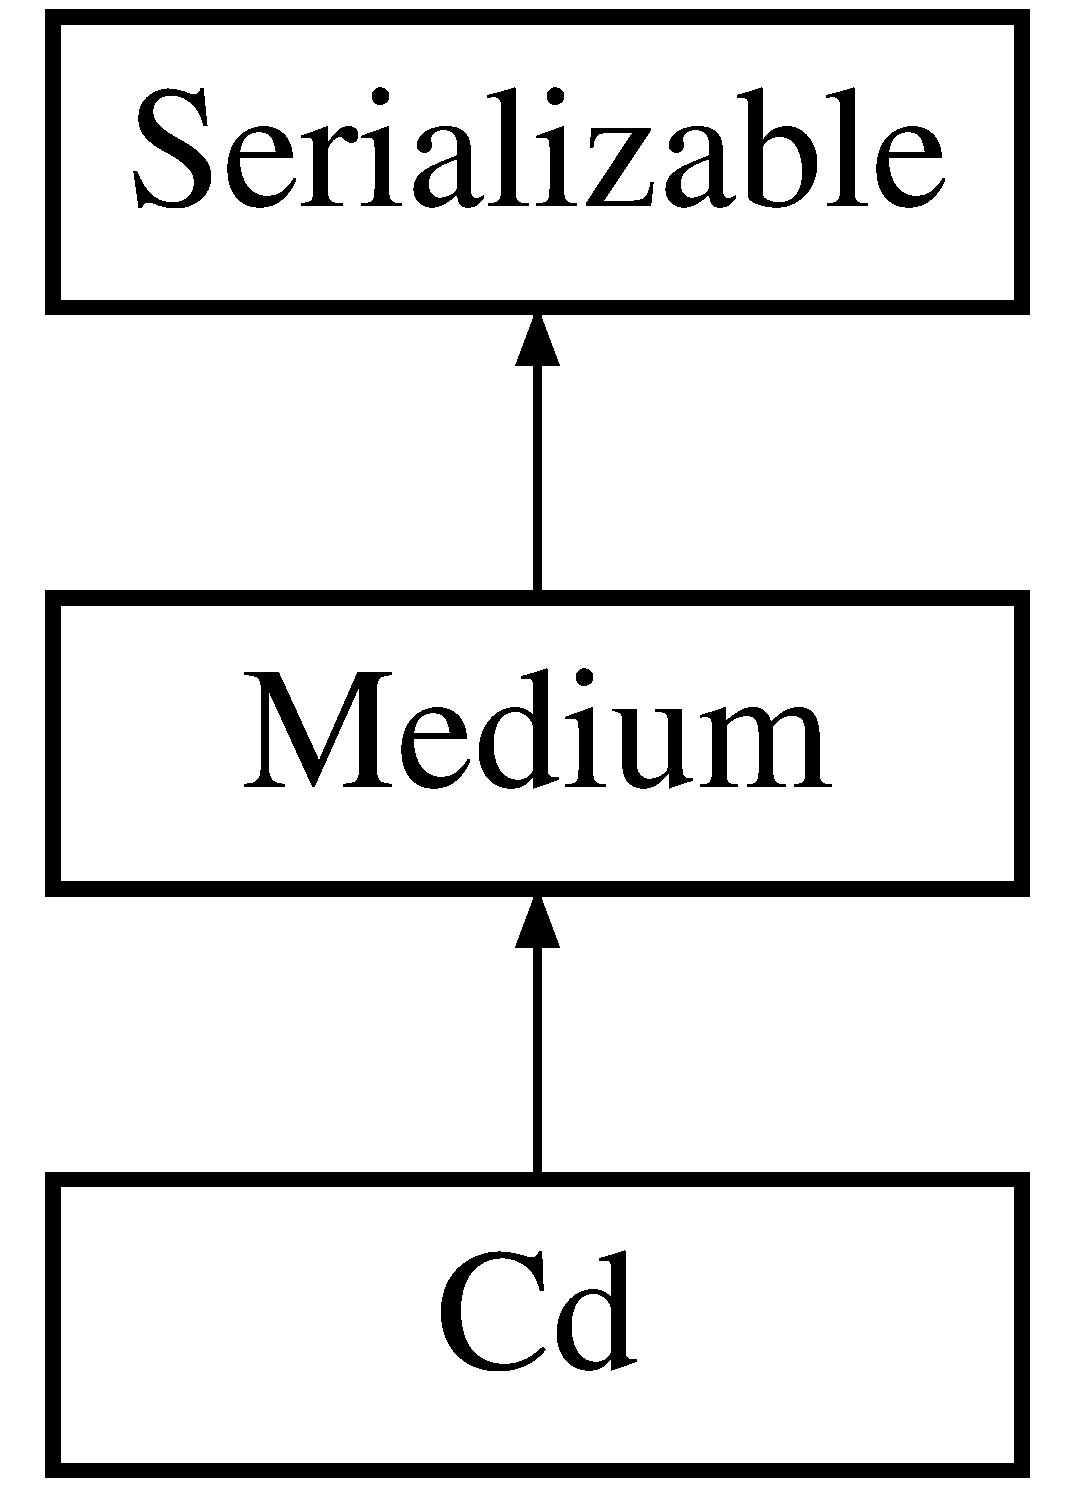
\includegraphics[height=3.000000cm]{classCd}
\end{center}
\end{figure}
\subsection*{Public Member Functions}
\begin{DoxyCompactItemize}
\item 
\hyperlink{classCd_a35f36899f88a65b28f3d85ccee2270f4}{Cd} (String titel, float preis, String interpret, \hyperlink{enumGenre}{Genre} genre)
\item 
\hyperlink{classCd_a22425fef5f31c3bae54cae2f81911d48}{Cd} (Random random)
\item 
String \hyperlink{classCd_af580a22ffbc326cb02e6c2fe7e7c9e55}{gib\-Interpret} ()
\item 
void \hyperlink{classCd_a4c685bbf10f484f98f61f1d206f99a4b}{setze\-Interpret} (String interpret)
\item 
\hyperlink{enumGenre}{Genre} \hyperlink{classCd_a5705282716e6b787a6d1f6236559df51}{gib\-Genre} ()
\item 
void \hyperlink{classCd_aa042d7c362dad5f4eaeedaaf71f64f5e}{setze\-Genre} (\hyperlink{enumGenre}{Genre} genre)
\item 
String \hyperlink{classCd_a597fea15f5c28cfab25b5d4352da9ab4}{to\-String} ()
\end{DoxyCompactItemize}


\subsection{Detailed Description}
\hyperlink{classCd}{Cd} ist eine Unterklasse von \hyperlink{classMedium}{Medium}. Es ergänzt \hyperlink{classMedium}{Medium} mit den für eine C\-D benötigten Felder und Eigenschaften.

\begin{DoxyAuthor}{Author}
Lukas Hodel 
\end{DoxyAuthor}


\subsection{Constructor \& Destructor Documentation}
\hypertarget{classCd_a35f36899f88a65b28f3d85ccee2270f4}{\index{Cd@{Cd}!Cd@{Cd}}
\index{Cd@{Cd}!Cd@{Cd}}
\subsubsection[{Cd}]{\setlength{\rightskip}{0pt plus 5cm}Cd.\-Cd (
\begin{DoxyParamCaption}
\item[{String}]{titel, }
\item[{float}]{preis, }
\item[{String}]{interpret, }
\item[{{\bf Genre}}]{genre}
\end{DoxyParamCaption}
)\hspace{0.3cm}{\ttfamily [inline]}}}\label{classCd_a35f36899f88a65b28f3d85ccee2270f4}
Der Konstruktor benoetigt alle Felder des Buches als Parameter


\begin{DoxyParams}{Parameters}
{\em titel} & String Titel der C\-D. \\
\hline
{\em preis} & float Preis der C\-D. \\
\hline
{\em interpret} & String Interpret der C\-D. \\
\hline
{\em genre} & genre der C\-D als Enum \hyperlink{enumGenre}{Genre}. \\
\hline
\end{DoxyParams}
\hypertarget{classCd_a22425fef5f31c3bae54cae2f81911d48}{\index{Cd@{Cd}!Cd@{Cd}}
\index{Cd@{Cd}!Cd@{Cd}}
\subsubsection[{Cd}]{\setlength{\rightskip}{0pt plus 5cm}Cd.\-Cd (
\begin{DoxyParamCaption}
\item[{Random}]{random}
\end{DoxyParamCaption}
)\hspace{0.3cm}{\ttfamily [inline]}}}\label{classCd_a22425fef5f31c3bae54cae2f81911d48}
Der Konstruktor benoetigt ein Random Objekt, dann werden die Felder automatisch gefüllt.


\begin{DoxyParams}{Parameters}
{\em random} & Objekt zur zufaelligen Wertegerierung. \\
\hline
\end{DoxyParams}


\subsection{Member Function Documentation}
\hypertarget{classCd_a5705282716e6b787a6d1f6236559df51}{\index{Cd@{Cd}!gib\-Genre@{gib\-Genre}}
\index{gib\-Genre@{gib\-Genre}!Cd@{Cd}}
\subsubsection[{gib\-Genre}]{\setlength{\rightskip}{0pt plus 5cm}{\bf Genre} Cd.\-gib\-Genre (
\begin{DoxyParamCaption}
{}
\end{DoxyParamCaption}
)\hspace{0.3cm}{\ttfamily [inline]}}}\label{classCd_a5705282716e6b787a6d1f6236559df51}
Gibt \hyperlink{enumGenre}{Genre} der \hyperlink{classCd}{Cd} zurueck. \hypertarget{classCd_af580a22ffbc326cb02e6c2fe7e7c9e55}{\index{Cd@{Cd}!gib\-Interpret@{gib\-Interpret}}
\index{gib\-Interpret@{gib\-Interpret}!Cd@{Cd}}
\subsubsection[{gib\-Interpret}]{\setlength{\rightskip}{0pt plus 5cm}String Cd.\-gib\-Interpret (
\begin{DoxyParamCaption}
{}
\end{DoxyParamCaption}
)\hspace{0.3cm}{\ttfamily [inline]}}}\label{classCd_af580a22ffbc326cb02e6c2fe7e7c9e55}
Gibt Interpret der \hyperlink{classCd}{Cd} zurueck. \hypertarget{classCd_aa042d7c362dad5f4eaeedaaf71f64f5e}{\index{Cd@{Cd}!setze\-Genre@{setze\-Genre}}
\index{setze\-Genre@{setze\-Genre}!Cd@{Cd}}
\subsubsection[{setze\-Genre}]{\setlength{\rightskip}{0pt plus 5cm}void Cd.\-setze\-Genre (
\begin{DoxyParamCaption}
\item[{{\bf Genre}}]{genre}
\end{DoxyParamCaption}
)\hspace{0.3cm}{\ttfamily [inline]}}}\label{classCd_aa042d7c362dad5f4eaeedaaf71f64f5e}
Setzt neues \hyperlink{enumGenre}{Genre} der \hyperlink{classCd}{Cd}.


\begin{DoxyParams}{Parameters}
{\em genre} & \hyperlink{enumGenre}{Genre} der \hyperlink{classCd}{Cd}. \\
\hline
\end{DoxyParams}
\hypertarget{classCd_a4c685bbf10f484f98f61f1d206f99a4b}{\index{Cd@{Cd}!setze\-Interpret@{setze\-Interpret}}
\index{setze\-Interpret@{setze\-Interpret}!Cd@{Cd}}
\subsubsection[{setze\-Interpret}]{\setlength{\rightskip}{0pt plus 5cm}void Cd.\-setze\-Interpret (
\begin{DoxyParamCaption}
\item[{String}]{interpret}
\end{DoxyParamCaption}
)\hspace{0.3cm}{\ttfamily [inline]}}}\label{classCd_a4c685bbf10f484f98f61f1d206f99a4b}
Setzt neuer Interpret.


\begin{DoxyParams}{Parameters}
{\em interpret} & neuer Interpret. \\
\hline
\end{DoxyParams}
\hypertarget{classCd_a597fea15f5c28cfab25b5d4352da9ab4}{\index{Cd@{Cd}!to\-String@{to\-String}}
\index{to\-String@{to\-String}!Cd@{Cd}}
\subsubsection[{to\-String}]{\setlength{\rightskip}{0pt plus 5cm}String Cd.\-to\-String (
\begin{DoxyParamCaption}
{}
\end{DoxyParamCaption}
)\hspace{0.3cm}{\ttfamily [inline]}}}\label{classCd_a597fea15f5c28cfab25b5d4352da9ab4}
Definiert wie die \hyperlink{classCd}{Cd} als String repraesentiert werden soll.

Format\-: C\-D 'Titel' von 'Interpret' \mbox{[}genre\mbox{]} 

The documentation for this class was generated from the following file\-:\begin{DoxyCompactItemize}
\item 
Cd.\-java\end{DoxyCompactItemize}

\hypertarget{classDvd}{\section{Dvd Class Reference}
\label{classDvd}\index{Dvd@{Dvd}}
}
Inheritance diagram for Dvd\-:\begin{figure}[H]
\begin{center}
\leavevmode
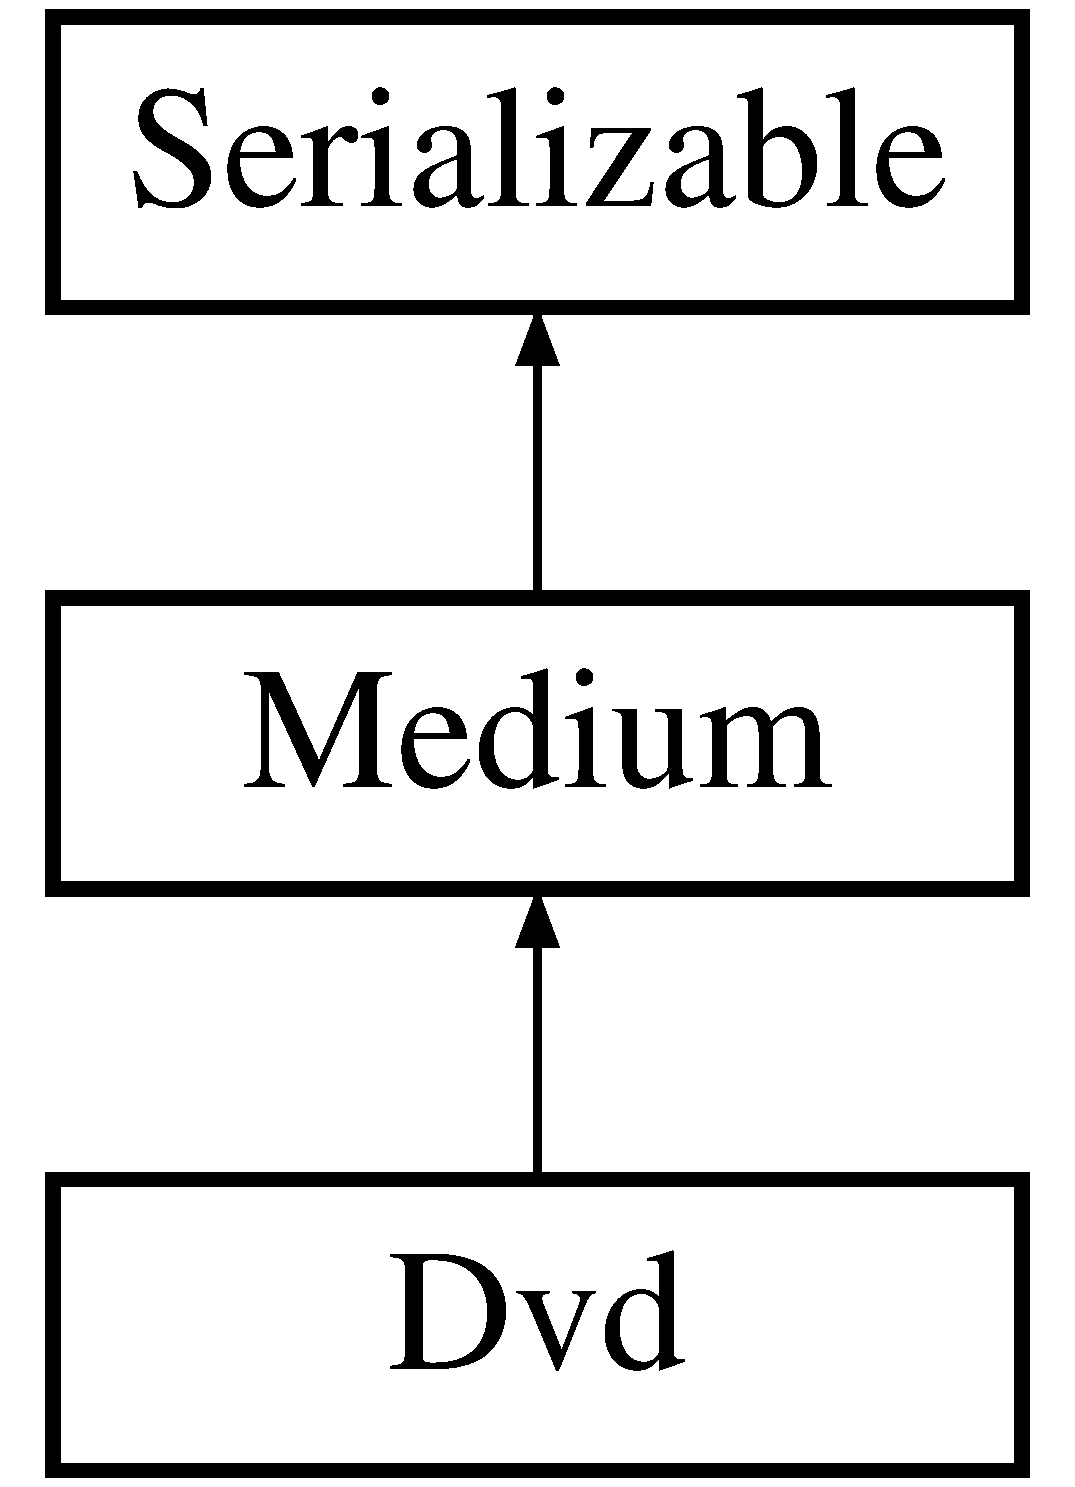
\includegraphics[height=3.000000cm]{classDvd}
\end{center}
\end{figure}
\subsection*{Public Member Functions}
\begin{DoxyCompactItemize}
\item 
\hyperlink{classDvd_a2d6d1fe33da6d6039f8cf8baee463291}{Dvd} (String titel, float preis, String regisseur, int freigabealter)
\item 
\hyperlink{classDvd_adb3ad96714865b09806c44e1538e5bf3}{Dvd} (Random random)
\item 
String \hyperlink{classDvd_a02b2a8ad9958fa39915f348811c84297}{gib\-Regisseur} ()
\item 
void \hyperlink{classDvd_a408943b8938726987c765ac9f472372c}{setze\-Regisseur} (String regisseur)
\item 
int \hyperlink{classDvd_a5a7c06f2d979fa7c092936ca429fa361}{gibfreigabealter} ()
\item 
void \hyperlink{classDvd_ac452a14d1d14f1b28d3b19f7b6532270}{setze\-Freigabealter} (int freigabealter)
\item 
String \hyperlink{classDvd_a646f663f014244c28ced8a20c6b0c49c}{to\-String} ()
\end{DoxyCompactItemize}


\subsection{Detailed Description}
\hyperlink{classDvd}{Dvd} ist eine Unterklasse von \hyperlink{classMedium}{Medium}. Es ergänzt \hyperlink{classMedium}{Medium} mit den für eine C\-D benötigten Felder und Eigenschaften.

\begin{DoxyAuthor}{Author}
Lukas Hodel 
\end{DoxyAuthor}


\subsection{Constructor \& Destructor Documentation}
\hypertarget{classDvd_a2d6d1fe33da6d6039f8cf8baee463291}{\index{Dvd@{Dvd}!Dvd@{Dvd}}
\index{Dvd@{Dvd}!Dvd@{Dvd}}
\subsubsection[{Dvd}]{\setlength{\rightskip}{0pt plus 5cm}Dvd.\-Dvd (
\begin{DoxyParamCaption}
\item[{String}]{titel, }
\item[{float}]{preis, }
\item[{String}]{regisseur, }
\item[{int}]{freigabealter}
\end{DoxyParamCaption}
)\hspace{0.3cm}{\ttfamily [inline]}}}\label{classDvd_a2d6d1fe33da6d6039f8cf8baee463291}
Der Konstruktor benoetigt alle Felder des Buches als Parameter


\begin{DoxyParams}{Parameters}
{\em preis} & float Preis der D\-V\-D. \\
\hline
{\em regisseur} & String Regisseur des Films. \\
\hline
{\em freigabealter} & int Freigabealter für den Film. \\
\hline
\end{DoxyParams}
\hypertarget{classDvd_adb3ad96714865b09806c44e1538e5bf3}{\index{Dvd@{Dvd}!Dvd@{Dvd}}
\index{Dvd@{Dvd}!Dvd@{Dvd}}
\subsubsection[{Dvd}]{\setlength{\rightskip}{0pt plus 5cm}Dvd.\-Dvd (
\begin{DoxyParamCaption}
\item[{Random}]{random}
\end{DoxyParamCaption}
)\hspace{0.3cm}{\ttfamily [inline]}}}\label{classDvd_adb3ad96714865b09806c44e1538e5bf3}
Der Konstruktor benoetigt ein Random Objekt, dann werden die Felder automatisch gefüllt.


\begin{DoxyParams}{Parameters}
{\em random} & Objekt zur zufaelligen Wertegerierung. \\
\hline
\end{DoxyParams}


\subsection{Member Function Documentation}
\hypertarget{classDvd_a5a7c06f2d979fa7c092936ca429fa361}{\index{Dvd@{Dvd}!gibfreigabealter@{gibfreigabealter}}
\index{gibfreigabealter@{gibfreigabealter}!Dvd@{Dvd}}
\subsubsection[{gibfreigabealter}]{\setlength{\rightskip}{0pt plus 5cm}int Dvd.\-gibfreigabealter (
\begin{DoxyParamCaption}
{}
\end{DoxyParamCaption}
)\hspace{0.3cm}{\ttfamily [inline]}}}\label{classDvd_a5a7c06f2d979fa7c092936ca429fa361}
Gibt Freigabealter zurueck. \hypertarget{classDvd_a02b2a8ad9958fa39915f348811c84297}{\index{Dvd@{Dvd}!gib\-Regisseur@{gib\-Regisseur}}
\index{gib\-Regisseur@{gib\-Regisseur}!Dvd@{Dvd}}
\subsubsection[{gib\-Regisseur}]{\setlength{\rightskip}{0pt plus 5cm}String Dvd.\-gib\-Regisseur (
\begin{DoxyParamCaption}
{}
\end{DoxyParamCaption}
)\hspace{0.3cm}{\ttfamily [inline]}}}\label{classDvd_a02b2a8ad9958fa39915f348811c84297}
Gibt Regisseur der \hyperlink{classCd}{Cd} zurueck. \hypertarget{classDvd_ac452a14d1d14f1b28d3b19f7b6532270}{\index{Dvd@{Dvd}!setze\-Freigabealter@{setze\-Freigabealter}}
\index{setze\-Freigabealter@{setze\-Freigabealter}!Dvd@{Dvd}}
\subsubsection[{setze\-Freigabealter}]{\setlength{\rightskip}{0pt plus 5cm}void Dvd.\-setze\-Freigabealter (
\begin{DoxyParamCaption}
\item[{int}]{freigabealter}
\end{DoxyParamCaption}
)\hspace{0.3cm}{\ttfamily [inline]}}}\label{classDvd_ac452a14d1d14f1b28d3b19f7b6532270}
Setzt neues Freigabealter der \hyperlink{classDvd}{Dvd}.


\begin{DoxyParams}{Parameters}
{\em freigabealter} & neues Freigabealter. \\
\hline
\end{DoxyParams}
\hypertarget{classDvd_a408943b8938726987c765ac9f472372c}{\index{Dvd@{Dvd}!setze\-Regisseur@{setze\-Regisseur}}
\index{setze\-Regisseur@{setze\-Regisseur}!Dvd@{Dvd}}
\subsubsection[{setze\-Regisseur}]{\setlength{\rightskip}{0pt plus 5cm}void Dvd.\-setze\-Regisseur (
\begin{DoxyParamCaption}
\item[{String}]{regisseur}
\end{DoxyParamCaption}
)\hspace{0.3cm}{\ttfamily [inline]}}}\label{classDvd_a408943b8938726987c765ac9f472372c}
Setzt neuen Regisseur der \hyperlink{classDvd}{Dvd}.


\begin{DoxyParams}{Parameters}
{\em regisseur} & neuer Regisseur. \\
\hline
\end{DoxyParams}
\hypertarget{classDvd_a646f663f014244c28ced8a20c6b0c49c}{\index{Dvd@{Dvd}!to\-String@{to\-String}}
\index{to\-String@{to\-String}!Dvd@{Dvd}}
\subsubsection[{to\-String}]{\setlength{\rightskip}{0pt plus 5cm}String Dvd.\-to\-String (
\begin{DoxyParamCaption}
{}
\end{DoxyParamCaption}
)\hspace{0.3cm}{\ttfamily [inline]}}}\label{classDvd_a646f663f014244c28ced8a20c6b0c49c}
Definiert wie die \hyperlink{classCd}{Cd} als String repraesentiert werden soll.

Format\-: D\-V\-D 'Titel' von 'Regisseur' (frei ab freigabealter). 

The documentation for this class was generated from the following file\-:\begin{DoxyCompactItemize}
\item 
Dvd.\-java\end{DoxyCompactItemize}

\hypertarget{enumGenre}{\section{Genre Enum Reference}
\label{enumGenre}\index{Genre@{Genre}}
}
\subsection*{Public Member Functions}
\begin{DoxyCompactItemize}
\item 
\hyperlink{enumGenre_a8f0f5830bdc68780662b85b2de8788dd}{Genre} (String genre)
\item 
String \hyperlink{enumGenre_a966802306a289298a9a11a6610cffeaa}{to\-String} ()
\end{DoxyCompactItemize}
\subsection*{Static Public Member Functions}
\begin{DoxyCompactItemize}
\item 
static \hyperlink{enumGenre}{Genre} \hyperlink{enumGenre_ae9eb554721c8e23706cf8f3042edb854}{gib\-Zufaellig} (Random random)
\end{DoxyCompactItemize}
\subsection*{Public Attributes}
\begin{DoxyCompactItemize}
\item 
\hyperlink{enumGenre_abeba5ef2f501e1284b2a64cc3b153153}{R\-O\-C\-K} =(\char`\"{}Rock\char`\"{})
\item 
\hyperlink{enumGenre_a68166334621841bdb574dc1fbe97f0b8}{P\-O\-P} =(\char`\"{}Pop\char`\"{})
\item 
\hyperlink{enumGenre_a78a8368dbd53da52a36348fe432eda31}{K\-L\-A\-S\-S\-I\-K} =(\char`\"{}Klassik\char`\"{})
\item 
\hyperlink{enumGenre_a920a44dbb49797e79965fddc177c36d5}{H\-I\-P\-H\-O\-P} =(\char`\"{}Hip\-Hop\char`\"{})
\item 
\hyperlink{enumGenre_a45892876ee0f75ebe59202cf7d57fc78}{M\-E\-T\-A\-L} =(\char`\"{}Metal\char`\"{})
\item 
\hyperlink{enumGenre_af7ee5c3305bd4ab99555c3c5bd92e1a9}{T\-E\-C\-H\-N\-O} =(\char`\"{}Techno\char`\"{})
\item 
\hyperlink{enumGenre_a987305efa37d1df58608a8635407add0}{J\-A\-Z\-Z} =(\char`\"{}Jazz\char`\"{})
\end{DoxyCompactItemize}


\subsection{Detailed Description}
Enum-\/\-Klasse mit den Musik-\/\-Genres der C\-Ds. Jedes \hyperlink{enumGenre}{Genre} wird mit einem String initialisiert, die die Ausgabe des Genres als String darstellt.

\begin{DoxyAuthor}{Author}
Lukas Hodel 
\end{DoxyAuthor}


\subsection{Constructor \& Destructor Documentation}
\hypertarget{enumGenre_a8f0f5830bdc68780662b85b2de8788dd}{\index{Genre@{Genre}!Genre@{Genre}}
\index{Genre@{Genre}!Genre@{Genre}}
\subsubsection[{Genre}]{\setlength{\rightskip}{0pt plus 5cm}Genre.\-Genre (
\begin{DoxyParamCaption}
\item[{String}]{genre}
\end{DoxyParamCaption}
)\hspace{0.3cm}{\ttfamily [inline]}}}\label{enumGenre_a8f0f5830bdc68780662b85b2de8788dd}
T\-O\-D\-O \-: !!! 

\subsection{Member Function Documentation}
\hypertarget{enumGenre_ae9eb554721c8e23706cf8f3042edb854}{\index{Genre@{Genre}!gib\-Zufaellig@{gib\-Zufaellig}}
\index{gib\-Zufaellig@{gib\-Zufaellig}!Genre@{Genre}}
\subsubsection[{gib\-Zufaellig}]{\setlength{\rightskip}{0pt plus 5cm}static {\bf Genre} Genre.\-gib\-Zufaellig (
\begin{DoxyParamCaption}
\item[{Random}]{random}
\end{DoxyParamCaption}
)\hspace{0.3cm}{\ttfamily [inline]}, {\ttfamily [static]}}}\label{enumGenre_ae9eb554721c8e23706cf8f3042edb854}
Gibt ein zufälliges \hyperlink{enumGenre}{Genre} zurück.

random Eine Random instanz.

\begin{DoxyReturn}{Returns}
ein zufälliges genre \hyperlink{enumGenre}{Genre}. 
\end{DoxyReturn}
\hypertarget{enumGenre_a966802306a289298a9a11a6610cffeaa}{\index{Genre@{Genre}!to\-String@{to\-String}}
\index{to\-String@{to\-String}!Genre@{Genre}}
\subsubsection[{to\-String}]{\setlength{\rightskip}{0pt plus 5cm}String Genre.\-to\-String (
\begin{DoxyParamCaption}
{}
\end{DoxyParamCaption}
)\hspace{0.3cm}{\ttfamily [inline]}}}\label{enumGenre_a966802306a289298a9a11a6610cffeaa}
Überschreibt \hyperlink{enumGenre_a966802306a289298a9a11a6610cffeaa}{to\-String()} damit der genre Stringwert zurückgegeben wird.

\begin{DoxyReturn}{Returns}
\hyperlink{enumGenre}{Genre} als String. 
\end{DoxyReturn}


\subsection{Member Data Documentation}
\hypertarget{enumGenre_a920a44dbb49797e79965fddc177c36d5}{\index{Genre@{Genre}!H\-I\-P\-H\-O\-P@{H\-I\-P\-H\-O\-P}}
\index{H\-I\-P\-H\-O\-P@{H\-I\-P\-H\-O\-P}!Genre@{Genre}}
\subsubsection[{H\-I\-P\-H\-O\-P}]{\setlength{\rightskip}{0pt plus 5cm}Genre.\-H\-I\-P\-H\-O\-P =(\char`\"{}Hip\-Hop\char`\"{})}}\label{enumGenre_a920a44dbb49797e79965fddc177c36d5}
\hyperlink{enumGenre}{Genre} Hip\-Hop \hypertarget{enumGenre_a987305efa37d1df58608a8635407add0}{\index{Genre@{Genre}!J\-A\-Z\-Z@{J\-A\-Z\-Z}}
\index{J\-A\-Z\-Z@{J\-A\-Z\-Z}!Genre@{Genre}}
\subsubsection[{J\-A\-Z\-Z}]{\setlength{\rightskip}{0pt plus 5cm}Genre.\-J\-A\-Z\-Z =(\char`\"{}Jazz\char`\"{})}}\label{enumGenre_a987305efa37d1df58608a8635407add0}
\hyperlink{enumGenre}{Genre} Jazz \hypertarget{enumGenre_a78a8368dbd53da52a36348fe432eda31}{\index{Genre@{Genre}!K\-L\-A\-S\-S\-I\-K@{K\-L\-A\-S\-S\-I\-K}}
\index{K\-L\-A\-S\-S\-I\-K@{K\-L\-A\-S\-S\-I\-K}!Genre@{Genre}}
\subsubsection[{K\-L\-A\-S\-S\-I\-K}]{\setlength{\rightskip}{0pt plus 5cm}Genre.\-K\-L\-A\-S\-S\-I\-K =(\char`\"{}Klassik\char`\"{})}}\label{enumGenre_a78a8368dbd53da52a36348fe432eda31}
\hyperlink{enumGenre}{Genre} Klassik \hypertarget{enumGenre_a45892876ee0f75ebe59202cf7d57fc78}{\index{Genre@{Genre}!M\-E\-T\-A\-L@{M\-E\-T\-A\-L}}
\index{M\-E\-T\-A\-L@{M\-E\-T\-A\-L}!Genre@{Genre}}
\subsubsection[{M\-E\-T\-A\-L}]{\setlength{\rightskip}{0pt plus 5cm}Genre.\-M\-E\-T\-A\-L =(\char`\"{}Metal\char`\"{})}}\label{enumGenre_a45892876ee0f75ebe59202cf7d57fc78}
\hyperlink{enumGenre}{Genre} Metal \hypertarget{enumGenre_a68166334621841bdb574dc1fbe97f0b8}{\index{Genre@{Genre}!P\-O\-P@{P\-O\-P}}
\index{P\-O\-P@{P\-O\-P}!Genre@{Genre}}
\subsubsection[{P\-O\-P}]{\setlength{\rightskip}{0pt plus 5cm}Genre.\-P\-O\-P =(\char`\"{}Pop\char`\"{})}}\label{enumGenre_a68166334621841bdb574dc1fbe97f0b8}
\hyperlink{enumGenre}{Genre} Pop \hypertarget{enumGenre_abeba5ef2f501e1284b2a64cc3b153153}{\index{Genre@{Genre}!R\-O\-C\-K@{R\-O\-C\-K}}
\index{R\-O\-C\-K@{R\-O\-C\-K}!Genre@{Genre}}
\subsubsection[{R\-O\-C\-K}]{\setlength{\rightskip}{0pt plus 5cm}Genre.\-R\-O\-C\-K =(\char`\"{}Rock\char`\"{})}}\label{enumGenre_abeba5ef2f501e1284b2a64cc3b153153}
\hyperlink{enumGenre}{Genre} Rock \hypertarget{enumGenre_af7ee5c3305bd4ab99555c3c5bd92e1a9}{\index{Genre@{Genre}!T\-E\-C\-H\-N\-O@{T\-E\-C\-H\-N\-O}}
\index{T\-E\-C\-H\-N\-O@{T\-E\-C\-H\-N\-O}!Genre@{Genre}}
\subsubsection[{T\-E\-C\-H\-N\-O}]{\setlength{\rightskip}{0pt plus 5cm}Genre.\-T\-E\-C\-H\-N\-O =(\char`\"{}Techno\char`\"{})}}\label{enumGenre_af7ee5c3305bd4ab99555c3c5bd92e1a9}
\hyperlink{enumGenre}{Genre} Techno 

The documentation for this enum was generated from the following file\-:\begin{DoxyCompactItemize}
\item 
Genre.\-java\end{DoxyCompactItemize}

\hypertarget{classMedienversandMain}{\section{Medienversand\-Main Class Reference}
\label{classMedienversandMain}\index{Medienversand\-Main@{Medienversand\-Main}}
}
\subsection*{Static Public Member Functions}
\begin{DoxyCompactItemize}
\item 
static void \hyperlink{classMedienversandMain_a2bae9e6e85f58239f993afa2c831ca65}{main} (String\mbox{[}$\,$\mbox{]} args)
\end{DoxyCompactItemize}
\subsection*{Static Public Attributes}
\begin{DoxyCompactItemize}
\item 
static final String \hyperlink{classMedienversandMain_a3e8118d08738afd15fe2bf18919b5834}{N\-A\-M\-E} = \char`\"{}Medienversand\-Main\char`\"{}
\end{DoxyCompactItemize}


\subsection{Detailed Description}
Simulation eines Medienversands der Buecher, C\-Ds und D\-V\-Ds vertreibt. Es werden fuer 365 Tage eine vom Benutzer gewuenschte Anzahl Medien zufaellig generiert und in die Dateien Medien.\-dat und Verkauf.\-dat geschrieben. Es kann danach fuer einen beliebigen Tag die Verkaufsdaten ausgegeben werden. Es handelt sich um ein Terminal Programm.

\begin{DoxyAuthor}{Author}
Lukas Hodel 
\end{DoxyAuthor}


\subsection{Member Function Documentation}
\hypertarget{classMedienversandMain_a2bae9e6e85f58239f993afa2c831ca65}{\index{Medienversand\-Main@{Medienversand\-Main}!main@{main}}
\index{main@{main}!MedienversandMain@{Medienversand\-Main}}
\subsubsection[{main}]{\setlength{\rightskip}{0pt plus 5cm}static void Medienversand\-Main.\-main (
\begin{DoxyParamCaption}
\item[{String\mbox{[}$\,$\mbox{]}}]{args}
\end{DoxyParamCaption}
)\hspace{0.3cm}{\ttfamily [inline]}, {\ttfamily [static]}}}\label{classMedienversandMain_a2bae9e6e85f58239f993afa2c831ca65}
Ueberprueft die uebergebenen Parameter und startet die Simulation, wenn die Paramter ok sind. Sonst wird eine Information ausgegeben, wie das Programm zu Benutzen ist.


\begin{DoxyParams}{Parameters}
{\em args} & Fuer die Simulation benoetigten Programmparameter. \\
\hline
\end{DoxyParams}


\subsection{Member Data Documentation}
\hypertarget{classMedienversandMain_a3e8118d08738afd15fe2bf18919b5834}{\index{Medienversand\-Main@{Medienversand\-Main}!N\-A\-M\-E@{N\-A\-M\-E}}
\index{N\-A\-M\-E@{N\-A\-M\-E}!MedienversandMain@{Medienversand\-Main}}
\subsubsection[{N\-A\-M\-E}]{\setlength{\rightskip}{0pt plus 5cm}final String Medienversand\-Main.\-N\-A\-M\-E = \char`\"{}Medienversand\-Main\char`\"{}\hspace{0.3cm}{\ttfamily [static]}}}\label{classMedienversandMain_a3e8118d08738afd15fe2bf18919b5834}
Name des Programmes. 

The documentation for this class was generated from the following file\-:\begin{DoxyCompactItemize}
\item 
Medienversand\-Main.\-java\end{DoxyCompactItemize}

\hypertarget{classMedium}{\section{Medium Class Reference}
\label{classMedium}\index{Medium@{Medium}}
}
Inheritance diagram for Medium\-:\begin{figure}[H]
\begin{center}
\leavevmode
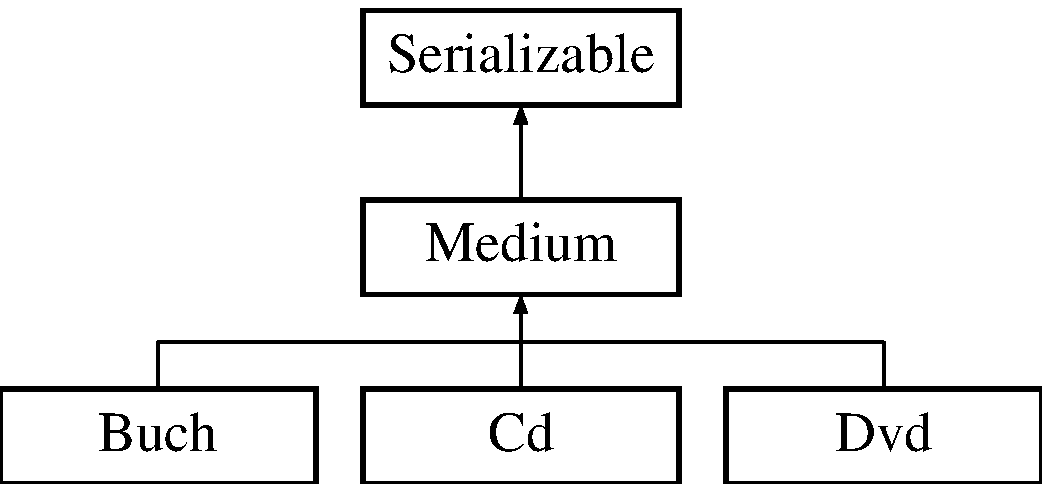
\includegraphics[height=3.000000cm]{classMedium}
\end{center}
\end{figure}
\subsection*{Public Member Functions}
\begin{DoxyCompactItemize}
\item 
\hyperlink{classMedium_a00549864dd88fc9c317504b7bd335701}{Medium} (String titel, float preis)
\item 
\hyperlink{classMedium_ac3b157358e6566a99d1de47c08836071}{Medium} (Random random)
\item 
String \hyperlink{classMedium_a07c01338a5027ca7b7034f0fd23fd196}{gib\-Titel} ()
\item 
void \hyperlink{classMedium_abc928f7f28de4a257a8be9e97d5e46d8}{setze\-Titel} (String titel)
\item 
float \hyperlink{classMedium_ac1434c472daefaf2af3775f957831919}{gib\-Preis} ()
\item 
void \hyperlink{classMedium_a7742ceb4b7ff5e850cb3f13afee4689f}{setze\-Preis} (float preis)
\item 
boolean \hyperlink{classMedium_a01d9c9999e0357603f822834978c2c5a}{equals} (Object obj)
\end{DoxyCompactItemize}


\subsection{Detailed Description}
Basisklasse für Mediumobjekte. Darin werden die von allen untertypen verwendeten Attributte definiert. Auch die Serialisierungsmethode wird hier definiert.

\begin{DoxyAuthor}{Author}
Lukas Hodel 
\end{DoxyAuthor}


\subsection{Constructor \& Destructor Documentation}
\hypertarget{classMedium_a00549864dd88fc9c317504b7bd335701}{\index{Medium@{Medium}!Medium@{Medium}}
\index{Medium@{Medium}!Medium@{Medium}}
\subsubsection[{Medium}]{\setlength{\rightskip}{0pt plus 5cm}Medium.\-Medium (
\begin{DoxyParamCaption}
\item[{String}]{titel, }
\item[{float}]{preis}
\end{DoxyParamCaption}
)\hspace{0.3cm}{\ttfamily [inline]}}}\label{classMedium_a00549864dd88fc9c317504b7bd335701}
Der Konstruktor benoetigt alle Felder des Mediums als Parameter


\begin{DoxyParams}{Parameters}
{\em titel} & Titel des Mediums. \\
\hline
{\em preis} & Preis des Mediums. \\
\hline
\end{DoxyParams}
\hypertarget{classMedium_ac3b157358e6566a99d1de47c08836071}{\index{Medium@{Medium}!Medium@{Medium}}
\index{Medium@{Medium}!Medium@{Medium}}
\subsubsection[{Medium}]{\setlength{\rightskip}{0pt plus 5cm}Medium.\-Medium (
\begin{DoxyParamCaption}
\item[{Random}]{random}
\end{DoxyParamCaption}
)\hspace{0.3cm}{\ttfamily [inline]}}}\label{classMedium_ac3b157358e6566a99d1de47c08836071}
Der Konstruktor benoetigt ein Random Objekt, dann werden die Felder automatisch gefüllt.


\begin{DoxyParams}{Parameters}
{\em random} & Objekt zur zufaelligen Wertegerierung. \\
\hline
\end{DoxyParams}


\subsection{Member Function Documentation}
\hypertarget{classMedium_a01d9c9999e0357603f822834978c2c5a}{\index{Medium@{Medium}!equals@{equals}}
\index{equals@{equals}!Medium@{Medium}}
\subsubsection[{equals}]{\setlength{\rightskip}{0pt plus 5cm}boolean Medium.\-equals (
\begin{DoxyParamCaption}
\item[{Object}]{obj}
\end{DoxyParamCaption}
)\hspace{0.3cm}{\ttfamily [inline]}}}\label{classMedium_a01d9c9999e0357603f822834978c2c5a}
Ueberschreibt die equals funktion so, dass ein \hyperlink{classMedium}{Medium} gleich ist, wenn der Titel, der Preis und die Klasse identisch sind. \hypertarget{classMedium_ac1434c472daefaf2af3775f957831919}{\index{Medium@{Medium}!gib\-Preis@{gib\-Preis}}
\index{gib\-Preis@{gib\-Preis}!Medium@{Medium}}
\subsubsection[{gib\-Preis}]{\setlength{\rightskip}{0pt plus 5cm}float Medium.\-gib\-Preis (
\begin{DoxyParamCaption}
{}
\end{DoxyParamCaption}
)\hspace{0.3cm}{\ttfamily [inline]}}}\label{classMedium_ac1434c472daefaf2af3775f957831919}
Gibt den Preis zurueck. \hypertarget{classMedium_a07c01338a5027ca7b7034f0fd23fd196}{\index{Medium@{Medium}!gib\-Titel@{gib\-Titel}}
\index{gib\-Titel@{gib\-Titel}!Medium@{Medium}}
\subsubsection[{gib\-Titel}]{\setlength{\rightskip}{0pt plus 5cm}String Medium.\-gib\-Titel (
\begin{DoxyParamCaption}
{}
\end{DoxyParamCaption}
)\hspace{0.3cm}{\ttfamily [inline]}}}\label{classMedium_a07c01338a5027ca7b7034f0fd23fd196}
Gibt den Titel zurueck. \hypertarget{classMedium_a7742ceb4b7ff5e850cb3f13afee4689f}{\index{Medium@{Medium}!setze\-Preis@{setze\-Preis}}
\index{setze\-Preis@{setze\-Preis}!Medium@{Medium}}
\subsubsection[{setze\-Preis}]{\setlength{\rightskip}{0pt plus 5cm}void Medium.\-setze\-Preis (
\begin{DoxyParamCaption}
\item[{float}]{preis}
\end{DoxyParamCaption}
)\hspace{0.3cm}{\ttfamily [inline]}}}\label{classMedium_a7742ceb4b7ff5e850cb3f13afee4689f}
Setzt den Preis neu.


\begin{DoxyParams}{Parameters}
{\em preis} & neuer Preis. \\
\hline
\end{DoxyParams}
\hypertarget{classMedium_abc928f7f28de4a257a8be9e97d5e46d8}{\index{Medium@{Medium}!setze\-Titel@{setze\-Titel}}
\index{setze\-Titel@{setze\-Titel}!Medium@{Medium}}
\subsubsection[{setze\-Titel}]{\setlength{\rightskip}{0pt plus 5cm}void Medium.\-setze\-Titel (
\begin{DoxyParamCaption}
\item[{String}]{titel}
\end{DoxyParamCaption}
)\hspace{0.3cm}{\ttfamily [inline]}}}\label{classMedium_abc928f7f28de4a257a8be9e97d5e46d8}
Setzt den Ttitel.


\begin{DoxyParams}{Parameters}
{\em titel} & neuer Titel. \\
\hline
\end{DoxyParams}


The documentation for this class was generated from the following file\-:\begin{DoxyCompactItemize}
\item 
Medium.\-java\end{DoxyCompactItemize}

\hypertarget{classVerkauf}{\section{Verkauf Class Reference}
\label{classVerkauf}\index{Verkauf@{Verkauf}}
}
Inheritance diagram for Verkauf\-:\begin{figure}[H]
\begin{center}
\leavevmode
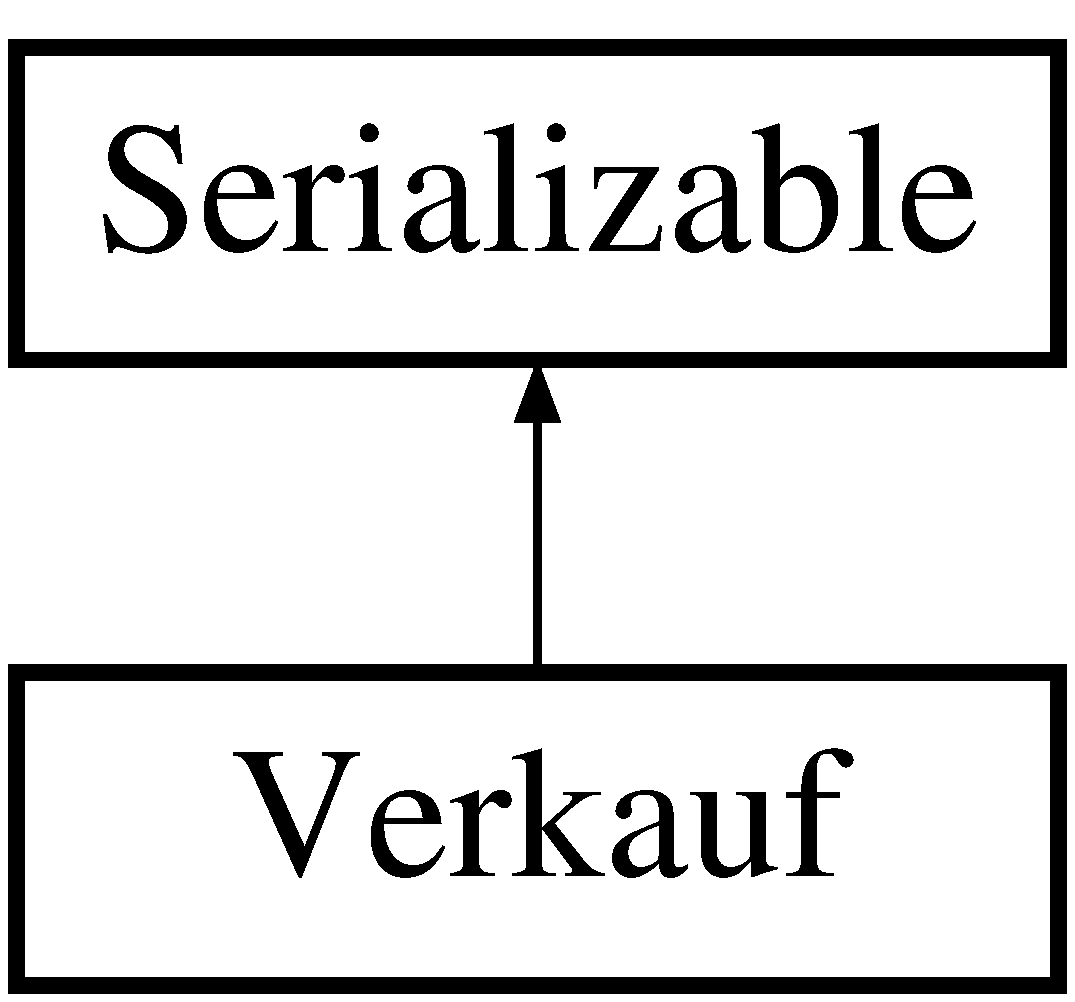
\includegraphics[height=2.000000cm]{classVerkauf}
\end{center}
\end{figure}
\subsection*{Public Member Functions}
\begin{DoxyCompactItemize}
\item 
\hyperlink{classVerkauf_a4c8bbcde7335b2484f8eea62e599fdda}{Verkauf} (int tag, \hyperlink{classMedium}{Medium} medium, int anzahl)
\item 
int \hyperlink{classVerkauf_a42cd9d706f948f243061a2bb063f625b}{gib\-Tag} ()
\item 
void \hyperlink{classVerkauf_a8507ef60bc4c288a67e0b7ad9cc61353}{setze\-Tag} (int tag)
\item 
\hyperlink{classMedium}{Medium} \hyperlink{classVerkauf_af628966d388e8d02bac45714f22d3d8f}{gib\-Medium} ()
\item 
void \hyperlink{classVerkauf_a609846c3a27057784339569a6d2fd880}{setze\-Medium} (\hyperlink{classMedium}{Medium} medium)
\item 
int \hyperlink{classVerkauf_ab5a8d75e43a4f0798a7860c74d56c300}{gib\-Anzahl} ()
\item 
void \hyperlink{classVerkauf_a236dcf8276e6609b05e236a99213b031}{setze\-Anzahl} (int anzahl)
\end{DoxyCompactItemize}


\subsection{Detailed Description}
\hyperlink{classBuch}{Buch} ist eine Unterklasse von \hyperlink{classMedium}{Medium}. Es ergänzt \hyperlink{classMedium}{Medium} mit den für ein \hyperlink{classBuch}{Buch} benötigten Felder und Eigenschaften.

\begin{DoxyAuthor}{Author}
Lukas Hodel 
\end{DoxyAuthor}


\subsection{Constructor \& Destructor Documentation}
\hypertarget{classVerkauf_a4c8bbcde7335b2484f8eea62e599fdda}{\index{Verkauf@{Verkauf}!Verkauf@{Verkauf}}
\index{Verkauf@{Verkauf}!Verkauf@{Verkauf}}
\subsubsection[{Verkauf}]{\setlength{\rightskip}{0pt plus 5cm}Verkauf.\-Verkauf (
\begin{DoxyParamCaption}
\item[{int}]{tag, }
\item[{{\bf Medium}}]{medium, }
\item[{int}]{anzahl}
\end{DoxyParamCaption}
)\hspace{0.3cm}{\ttfamily [inline]}}}\label{classVerkauf_a4c8bbcde7335b2484f8eea62e599fdda}
Anzahl wie oft das \hyperlink{classMedium}{Medium} an dem Tag verkauft wurde  Der Konstruktor benoetigt alle Felder des Verkaufs.


\begin{DoxyParams}{Parameters}
{\em tag} & Tag an welchem verkauft wurde. \\
\hline
{\em medium} & das verkaufte \hyperlink{classMedium}{Medium}. \\
\hline
{\em anzahl} & die anzahl, wie oft das \hyperlink{classMedium}{Medium} verkauft wurde. \\
\hline
\end{DoxyParams}


\subsection{Member Function Documentation}
\hypertarget{classVerkauf_ab5a8d75e43a4f0798a7860c74d56c300}{\index{Verkauf@{Verkauf}!gib\-Anzahl@{gib\-Anzahl}}
\index{gib\-Anzahl@{gib\-Anzahl}!Verkauf@{Verkauf}}
\subsubsection[{gib\-Anzahl}]{\setlength{\rightskip}{0pt plus 5cm}int Verkauf.\-gib\-Anzahl (
\begin{DoxyParamCaption}
{}
\end{DoxyParamCaption}
)\hspace{0.3cm}{\ttfamily [inline]}}}\label{classVerkauf_ab5a8d75e43a4f0798a7860c74d56c300}
Gibt die Anzahl zurueck wie oft das \hyperlink{classMedium}{Medium} verkauft wurde. \hypertarget{classVerkauf_af628966d388e8d02bac45714f22d3d8f}{\index{Verkauf@{Verkauf}!gib\-Medium@{gib\-Medium}}
\index{gib\-Medium@{gib\-Medium}!Verkauf@{Verkauf}}
\subsubsection[{gib\-Medium}]{\setlength{\rightskip}{0pt plus 5cm}{\bf Medium} Verkauf.\-gib\-Medium (
\begin{DoxyParamCaption}
{}
\end{DoxyParamCaption}
)\hspace{0.3cm}{\ttfamily [inline]}}}\label{classVerkauf_af628966d388e8d02bac45714f22d3d8f}
Gibt das \hyperlink{classMedium}{Medium} zurueck welches verkauft wurde. \hypertarget{classVerkauf_a42cd9d706f948f243061a2bb063f625b}{\index{Verkauf@{Verkauf}!gib\-Tag@{gib\-Tag}}
\index{gib\-Tag@{gib\-Tag}!Verkauf@{Verkauf}}
\subsubsection[{gib\-Tag}]{\setlength{\rightskip}{0pt plus 5cm}int Verkauf.\-gib\-Tag (
\begin{DoxyParamCaption}
{}
\end{DoxyParamCaption}
)\hspace{0.3cm}{\ttfamily [inline]}}}\label{classVerkauf_a42cd9d706f948f243061a2bb063f625b}
Gibt den Verkaufstag zurueck. \hypertarget{classVerkauf_a236dcf8276e6609b05e236a99213b031}{\index{Verkauf@{Verkauf}!setze\-Anzahl@{setze\-Anzahl}}
\index{setze\-Anzahl@{setze\-Anzahl}!Verkauf@{Verkauf}}
\subsubsection[{setze\-Anzahl}]{\setlength{\rightskip}{0pt plus 5cm}void Verkauf.\-setze\-Anzahl (
\begin{DoxyParamCaption}
\item[{int}]{anzahl}
\end{DoxyParamCaption}
)\hspace{0.3cm}{\ttfamily [inline]}}}\label{classVerkauf_a236dcf8276e6609b05e236a99213b031}
Setze die anzahl des Verkaufs.


\begin{DoxyParams}{Parameters}
{\em anzahl} & Anzahl wie oft das \hyperlink{classMedium}{Medium} verkauft wurde. \\
\hline
\end{DoxyParams}
\hypertarget{classVerkauf_a609846c3a27057784339569a6d2fd880}{\index{Verkauf@{Verkauf}!setze\-Medium@{setze\-Medium}}
\index{setze\-Medium@{setze\-Medium}!Verkauf@{Verkauf}}
\subsubsection[{setze\-Medium}]{\setlength{\rightskip}{0pt plus 5cm}void Verkauf.\-setze\-Medium (
\begin{DoxyParamCaption}
\item[{{\bf Medium}}]{medium}
\end{DoxyParamCaption}
)\hspace{0.3cm}{\ttfamily [inline]}}}\label{classVerkauf_a609846c3a27057784339569a6d2fd880}
Setze das verkaufte \hyperlink{classMedium}{Medium}


\begin{DoxyParams}{Parameters}
{\em anzahl} & Anzahl wie oft das \hyperlink{classMedium}{Medium} verkauft wurde. \\
\hline
\end{DoxyParams}
\hypertarget{classVerkauf_a8507ef60bc4c288a67e0b7ad9cc61353}{\index{Verkauf@{Verkauf}!setze\-Tag@{setze\-Tag}}
\index{setze\-Tag@{setze\-Tag}!Verkauf@{Verkauf}}
\subsubsection[{setze\-Tag}]{\setlength{\rightskip}{0pt plus 5cm}void Verkauf.\-setze\-Tag (
\begin{DoxyParamCaption}
\item[{int}]{tag}
\end{DoxyParamCaption}
)\hspace{0.3cm}{\ttfamily [inline]}}}\label{classVerkauf_a8507ef60bc4c288a67e0b7ad9cc61353}
Setze den Tag an welchem das \hyperlink{classMedium}{Medium} verkauft wurde.


\begin{DoxyParams}{Parameters}
{\em tag} & verkaufstag. \\
\hline
\end{DoxyParams}


The documentation for this class was generated from the following file\-:\begin{DoxyCompactItemize}
\item 
Verkauf.\-java\end{DoxyCompactItemize}

\hypertarget{classVerkaufPacket}{\section{Verkauf\-Packet Class Reference}
\label{classVerkaufPacket}\index{Verkauf\-Packet@{Verkauf\-Packet}}
}
Inheritance diagram for Verkauf\-Packet\-:\begin{figure}[H]
\begin{center}
\leavevmode
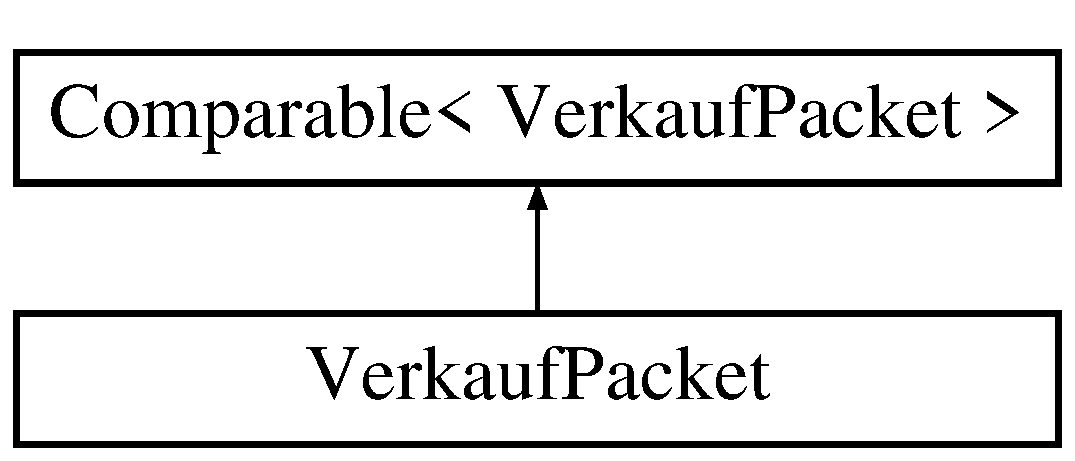
\includegraphics[height=2.000000cm]{classVerkaufPacket}
\end{center}
\end{figure}
\subsection*{Public Member Functions}
\begin{DoxyCompactItemize}
\item 
\hyperlink{classVerkaufPacket_a3386da111f7c9f1dfcc30911b0d7a33b}{Verkauf\-Packet} (\hyperlink{classMedium}{Medium} medium, int anzahl)
\item 
int \hyperlink{classVerkaufPacket_a6abe59e3f891d2b62b52ee61a4264325}{gib\-Anzahl} ()
\item 
void \hyperlink{classVerkaufPacket_a61f352d1a9bfd77eaf51176af334af7a}{setze\-Anzahl} (int anzahl)
\item 
\hyperlink{classMedium}{Medium} \hyperlink{classVerkaufPacket_a22d6fae8a2cbd3dbb7b258bf24d9e99d}{gib\-Medium} ()
\item 
void \hyperlink{classVerkaufPacket_a2ccb495d227ec9da75b80e53bcf0cc72}{setze\-Medium} (\hyperlink{classMedium}{Medium} medium)
\item 
float \hyperlink{classVerkaufPacket_a27dc0ed95b66b8fb573f9f1ebddc564e}{gib\-Preis} ()
\item 
float \hyperlink{classVerkaufPacket_a2f1e53843d2552c1d0a8dc4558758c87}{gib\-Gesamt\-Preis} ()
\item 
boolean \hyperlink{classVerkaufPacket_adbe07c2a07ed9a1ed511b34da6279601}{equals} (Object obj)
\item 
int \hyperlink{classVerkaufPacket_a2a0a506d856443a33ed3b2b5d25ba2bb}{compare\-To} (\hyperlink{classVerkaufPacket}{Verkauf\-Packet} gast)
\end{DoxyCompactItemize}


\subsection{Detailed Description}
\hyperlink{classBuch}{Buch} ist eine Unterklasse von \hyperlink{classMedium}{Medium}. Es ergänzt \hyperlink{classMedium}{Medium} mit den für ein \hyperlink{classBuch}{Buch} benötigten Felder und Eigenschaften.

\begin{DoxyAuthor}{Author}
Lukas Hodel 
\end{DoxyAuthor}


\subsection{Constructor \& Destructor Documentation}
\hypertarget{classVerkaufPacket_a3386da111f7c9f1dfcc30911b0d7a33b}{\index{Verkauf\-Packet@{Verkauf\-Packet}!Verkauf\-Packet@{Verkauf\-Packet}}
\index{Verkauf\-Packet@{Verkauf\-Packet}!VerkaufPacket@{Verkauf\-Packet}}
\subsubsection[{Verkauf\-Packet}]{\setlength{\rightskip}{0pt plus 5cm}Verkauf\-Packet.\-Verkauf\-Packet (
\begin{DoxyParamCaption}
\item[{{\bf Medium}}]{medium, }
\item[{int}]{anzahl}
\end{DoxyParamCaption}
)\hspace{0.3cm}{\ttfamily [inline]}}}\label{classVerkaufPacket_a3386da111f7c9f1dfcc30911b0d7a33b}
Der Konstruktor benoetigt alle Felder des Buches als Parameter


\begin{DoxyParams}{Parameters}
{\em titel} & String Titel des Buches. \\
\hline
{\em preis} & Float Preis des Buches. \\
\hline
{\em author} & String Author des Buches. \\
\hline
{\em hardcover} & boolean ob hardcover oder nicht. \\
\hline
\end{DoxyParams}


\subsection{Member Function Documentation}
\hypertarget{classVerkaufPacket_a2a0a506d856443a33ed3b2b5d25ba2bb}{\index{Verkauf\-Packet@{Verkauf\-Packet}!compare\-To@{compare\-To}}
\index{compare\-To@{compare\-To}!VerkaufPacket@{Verkauf\-Packet}}
\subsubsection[{compare\-To}]{\setlength{\rightskip}{0pt plus 5cm}int Verkauf\-Packet.\-compare\-To (
\begin{DoxyParamCaption}
\item[{{\bf Verkauf\-Packet}}]{gast}
\end{DoxyParamCaption}
)\hspace{0.3cm}{\ttfamily [inline]}}}\label{classVerkaufPacket_a2a0a506d856443a33ed3b2b5d25ba2bb}
Ueberschreibt die Methode compare\-To des interface Comparable. Definiert die Sortierreihenfolge.


\begin{DoxyParams}{Parameters}
{\em gast} & Das Gastobjekt mit welchem verglichen wird.\\
\hline
\end{DoxyParams}
\begin{DoxyReturn}{Returns}
Int 0 = gleich, 1 = groesser, -\/1 = kleiner 
\end{DoxyReturn}
\hypertarget{classVerkaufPacket_adbe07c2a07ed9a1ed511b34da6279601}{\index{Verkauf\-Packet@{Verkauf\-Packet}!equals@{equals}}
\index{equals@{equals}!VerkaufPacket@{Verkauf\-Packet}}
\subsubsection[{equals}]{\setlength{\rightskip}{0pt plus 5cm}boolean Verkauf\-Packet.\-equals (
\begin{DoxyParamCaption}
\item[{Object}]{obj}
\end{DoxyParamCaption}
)\hspace{0.3cm}{\ttfamily [inline]}}}\label{classVerkaufPacket_adbe07c2a07ed9a1ed511b34da6279601}
Definiert die Gleichheit eines \hyperlink{classVerkaufPacket}{Verkauf\-Packet}.


\begin{DoxyParams}{Parameters}
{\em obj} & Objekt mit welchem verglichen wird.\\
\hline
\end{DoxyParams}
\begin{DoxyReturn}{Returns}
boolean ob gleich oder nicht. 
\end{DoxyReturn}
\hypertarget{classVerkaufPacket_a6abe59e3f891d2b62b52ee61a4264325}{\index{Verkauf\-Packet@{Verkauf\-Packet}!gib\-Anzahl@{gib\-Anzahl}}
\index{gib\-Anzahl@{gib\-Anzahl}!VerkaufPacket@{Verkauf\-Packet}}
\subsubsection[{gib\-Anzahl}]{\setlength{\rightskip}{0pt plus 5cm}int Verkauf\-Packet.\-gib\-Anzahl (
\begin{DoxyParamCaption}
{}
\end{DoxyParamCaption}
)\hspace{0.3cm}{\ttfamily [inline]}}}\label{classVerkaufPacket_a6abe59e3f891d2b62b52ee61a4264325}
Gibt Anzahl zurueck. Wie oft wurde das \hyperlink{classMedium}{Medium} verkauft.

\begin{DoxyReturn}{Returns}
anzahl wie oft das \hyperlink{classMedium}{Medium} verkauft wurde. 
\end{DoxyReturn}
\hypertarget{classVerkaufPacket_a2f1e53843d2552c1d0a8dc4558758c87}{\index{Verkauf\-Packet@{Verkauf\-Packet}!gib\-Gesamt\-Preis@{gib\-Gesamt\-Preis}}
\index{gib\-Gesamt\-Preis@{gib\-Gesamt\-Preis}!VerkaufPacket@{Verkauf\-Packet}}
\subsubsection[{gib\-Gesamt\-Preis}]{\setlength{\rightskip}{0pt plus 5cm}float Verkauf\-Packet.\-gib\-Gesamt\-Preis (
\begin{DoxyParamCaption}
{}
\end{DoxyParamCaption}
)\hspace{0.3cm}{\ttfamily [inline]}}}\label{classVerkaufPacket_a2f1e53843d2552c1d0a8dc4558758c87}
Gibt der gesamte Verkaufspreis zurueck.

\begin{DoxyReturn}{Returns}
der gesamte Preis. Anzahl $\ast$ Preis. 
\end{DoxyReturn}
\hypertarget{classVerkaufPacket_a22d6fae8a2cbd3dbb7b258bf24d9e99d}{\index{Verkauf\-Packet@{Verkauf\-Packet}!gib\-Medium@{gib\-Medium}}
\index{gib\-Medium@{gib\-Medium}!VerkaufPacket@{Verkauf\-Packet}}
\subsubsection[{gib\-Medium}]{\setlength{\rightskip}{0pt plus 5cm}{\bf Medium} Verkauf\-Packet.\-gib\-Medium (
\begin{DoxyParamCaption}
{}
\end{DoxyParamCaption}
)\hspace{0.3cm}{\ttfamily [inline]}}}\label{classVerkaufPacket_a22d6fae8a2cbd3dbb7b258bf24d9e99d}
Gibt verkauftes \hyperlink{classMedium}{Medium} zurueck.

\begin{DoxyReturn}{Returns}
das verkaufte \hyperlink{classMedium}{Medium}. 
\end{DoxyReturn}
\hypertarget{classVerkaufPacket_a27dc0ed95b66b8fb573f9f1ebddc564e}{\index{Verkauf\-Packet@{Verkauf\-Packet}!gib\-Preis@{gib\-Preis}}
\index{gib\-Preis@{gib\-Preis}!VerkaufPacket@{Verkauf\-Packet}}
\subsubsection[{gib\-Preis}]{\setlength{\rightskip}{0pt plus 5cm}float Verkauf\-Packet.\-gib\-Preis (
\begin{DoxyParamCaption}
{}
\end{DoxyParamCaption}
)\hspace{0.3cm}{\ttfamily [inline]}}}\label{classVerkaufPacket_a27dc0ed95b66b8fb573f9f1ebddc564e}
Gibt verkaufspreis pro \hyperlink{classMedium}{Medium} zurueck.

\begin{DoxyReturn}{Returns}
Einzelpreis des Mediums. 
\end{DoxyReturn}
\hypertarget{classVerkaufPacket_a61f352d1a9bfd77eaf51176af334af7a}{\index{Verkauf\-Packet@{Verkauf\-Packet}!setze\-Anzahl@{setze\-Anzahl}}
\index{setze\-Anzahl@{setze\-Anzahl}!VerkaufPacket@{Verkauf\-Packet}}
\subsubsection[{setze\-Anzahl}]{\setlength{\rightskip}{0pt plus 5cm}void Verkauf\-Packet.\-setze\-Anzahl (
\begin{DoxyParamCaption}
\item[{int}]{anzahl}
\end{DoxyParamCaption}
)\hspace{0.3cm}{\ttfamily [inline]}}}\label{classVerkaufPacket_a61f352d1a9bfd77eaf51176af334af7a}
Setzt neue Anzahl an Medien.


\begin{DoxyParams}{Parameters}
{\em anzahl} & neue Anzahl Medien im Packet. \\
\hline
\end{DoxyParams}
\hypertarget{classVerkaufPacket_a2ccb495d227ec9da75b80e53bcf0cc72}{\index{Verkauf\-Packet@{Verkauf\-Packet}!setze\-Medium@{setze\-Medium}}
\index{setze\-Medium@{setze\-Medium}!VerkaufPacket@{Verkauf\-Packet}}
\subsubsection[{setze\-Medium}]{\setlength{\rightskip}{0pt plus 5cm}void Verkauf\-Packet.\-setze\-Medium (
\begin{DoxyParamCaption}
\item[{{\bf Medium}}]{medium}
\end{DoxyParamCaption}
)\hspace{0.3cm}{\ttfamily [inline]}}}\label{classVerkaufPacket_a2ccb495d227ec9da75b80e53bcf0cc72}
Setzt neues \hyperlink{classMedium}{Medium} welches Verkauft wurde.


\begin{DoxyParams}{Parameters}
{\em anzahl} & neue Anzahl Medien im Packet. \\
\hline
\end{DoxyParams}


The documentation for this class was generated from the following file\-:\begin{DoxyCompactItemize}
\item 
Verkauf\-Packet.\-java\end{DoxyCompactItemize}

%--- End generated contents ---

% Index
\newpage
\phantomsection
\addcontentsline{toc}{part}{Index}
\printindex

\end{document}
